\documentclass[a4paper,11pt]{article}
\usepackage[T1]{fontenc}
\usepackage[utf8]{inputenc}
\usepackage{graphicx}
\usepackage{rviewport}
\usepackage{xcolor}
\usepackage{siunitx}
\usepackage{booktabs}
\usepackage[left=30mm,right=30mm,top=30mm,bottom=45mm]{geometry}
\usepackage[%
        bookmarksnumbered=true,
        colorlinks=true,
        linkcolor=cyan!50!blue,
        citecolor=violet,
        urlcolor=purple,
    ]{hyperref}

\title{Including Graphics In Documents}
\author{Raphael Frey <\href{mailto:webmaster@alpenwasser.net}{\nolinkurl{webmaster@alpenwasser.net}}>}

\newcommand\code[1]{\texttt{#1}}

% ************************************************************************** % 
\begin{document}
% ************************************************************************** % 

\maketitle

\begin{abstract}
    Including  graphics in  a  document  is a  very  common  task. One of  the
    easier  ways,  and  the  one  I   use  most  frequently,  is  to  use  the
    \code{graphicx} package\footnotemark.  This  document presents some common
    examples on  how to use  it. For demonstration  purposes, we are  going to
    be  using  two images: A  PDF  document  of size  \SI{8}{\centi\meter}  by
    \SI{8}{\centi\meter}, and a  PNG version of the same  image with different
    dimensions (see Section \ref{sec:true-size}).
\end{abstract}

\footnotetext{%
    For            the            full           documentation,            see
    \href{http://ctan.org/pkg/graphicx}{\nolinkurl{http://ctan.org/pkg/graphicx}}}

\tableofcontents


% -------------------------------------------------------------------------- % 
\newpage
\section{Including an Image Without Additional Options}
% -------------------------------------------------------------------------- % 

The following code includes the PDF file as-is as an image\footnotemark:

\footnotetext{%
    \emph{Note:} The extension is  not strictly necessary.  But  in this case,
    since we have  both a file \code{grid8cm.pdf}  and \code{grid8cm.png}, the
    PNG version would  get included (at least on my  machine) if the extension
    is omitted. Personally, I never omit the extension.}

\begin{verbatim}
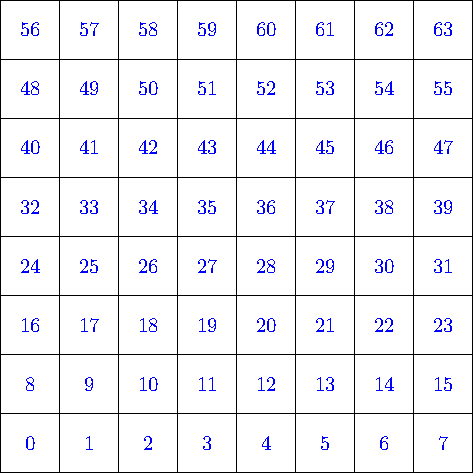
\includegraphics{images/grid8cm.pdf}
\end{verbatim}
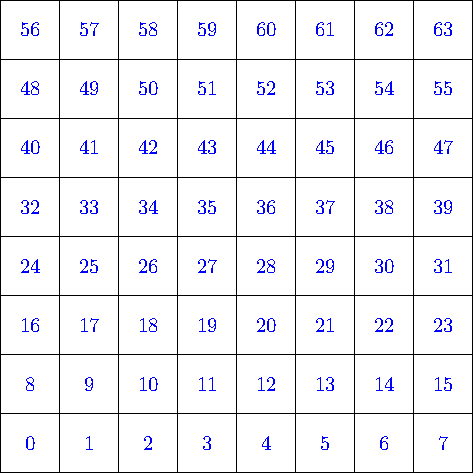
\includegraphics{images/grid8cm.pdf}


% -------------------------------------------------------------------------- % 
\newpage
\section{Centering a Picture}
% -------------------------------------------------------------------------- % 

We can center the included picture by using\footnotemark:

\footnotetext{
    In the common case of using floats via the \code{figure} environment, this
    code would  look a bit  different, but  we're primarily interested  in the
    mechanism  of  including graphics  here,  not  the  rabbit hole  which  is
    floats. That's for a different time.}

\begin{verbatim}
\begin{center}
    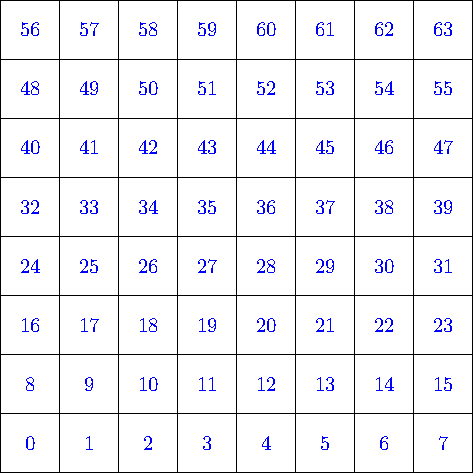
\includegraphics{images/grid8cm.pdf}
\end{center}
\end{verbatim}

\begin{center}
    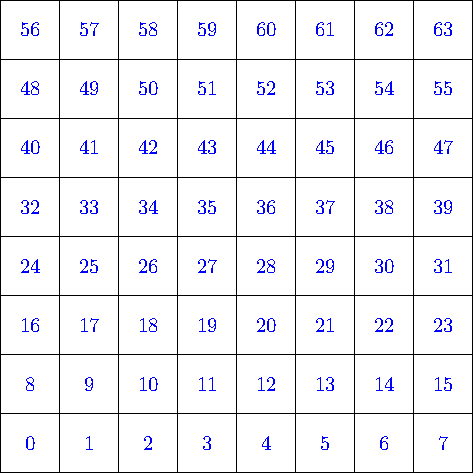
\includegraphics{images/grid8cm.pdf}
\end{center}


% -------------------------------------------------------------------------- % 
\section{Scaling a Picture}
% -------------------------------------------------------------------------- % 

Scaling  a  picture  (or text,  for  that  matter)  can  be achieved  via  the
\code{scalebox}  command,  which scales  by  a  horizontal, and  optionally  a
vertical, factor:

\begin{verbatim}
\scalebox{0.75}[0.5]{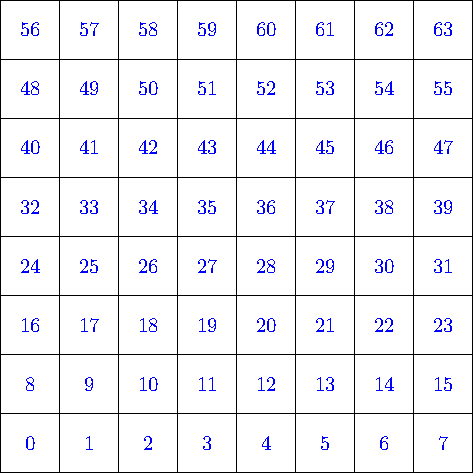
\includegraphics{images/grid8cm.pdf}}
\end{verbatim}

\scalebox{0.75}[0.5]{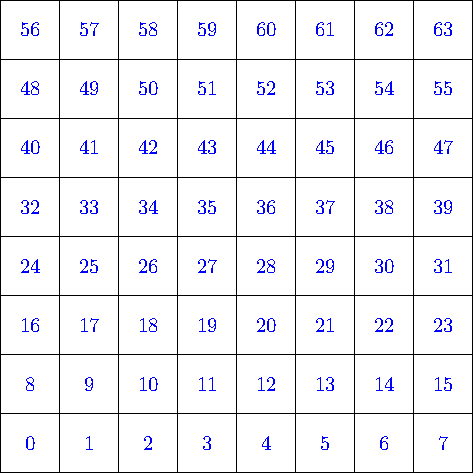
\includegraphics{images/grid8cm.pdf}}

\newpage
Negative factors work as well\footnotemark:

\footnotetext{%
    There also exists the  \code{\textbackslash{}reflectbox} command, which is
    an abbreviation for \code{\textbackslash{}scalebox\{-1\}[1]}.}

\begin{verbatim}
\scalebox{-0.5}[-0.5]{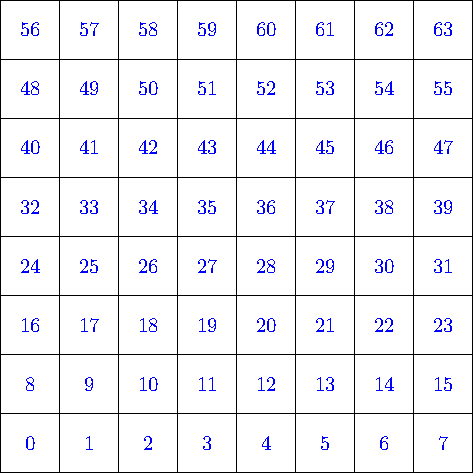
\includegraphics{images/grid8cm.pdf}}
\end{verbatim}

\scalebox{-0.5}[-0.5]{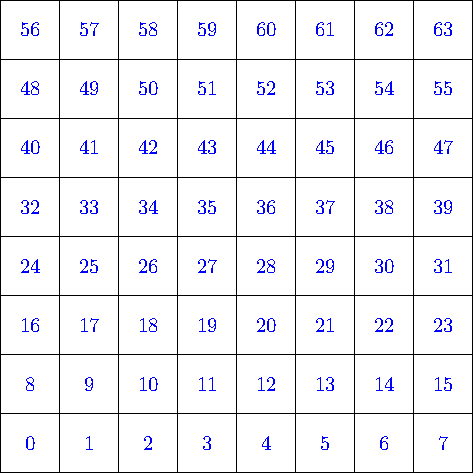
\includegraphics{images/grid8cm.pdf}}

\vspace{1em}

Alternatively,    one    may    specify    a    desired    size    with    the
\code{\textbackslash{}resizebox} command:

\begin{verbatim}
\resizebox{4cm}{!}{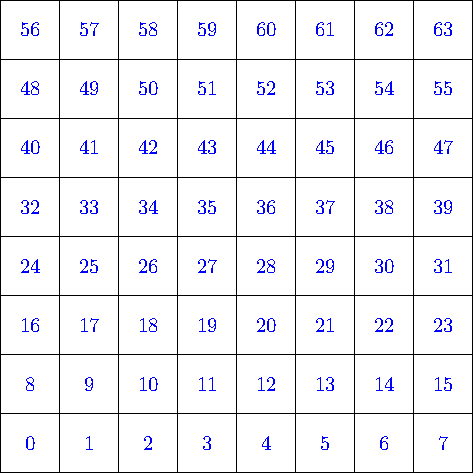
\includegraphics{images/grid8cm.pdf}}
\end{verbatim}

The  \code{!}   in  the  second  argument   means  that  the  box   should  be
scaled  proportionally  by whatever  factor  results  from the  other  length.
\code{\textbackslash{}resizebox\{!\}\{4cm\}}  would yield  the same  result in
this instance, as would \code{\textbackslash{}resizebox\{4cm\}\{4cm\}}.

\vspace{1em}

\resizebox{4cm}{!}{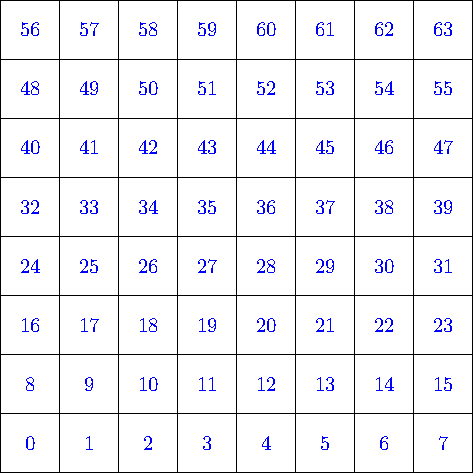
\includegraphics{images/grid8cm.pdf}}

\vspace{1em}

Note that everything inside these  boxes is scaled, including text. This means
that  if  consistent font  sizes  are  desired  throughout a   document,  this
approach  is  not optimal. Such  a  situation  might  for example  arise  when
including a Ti\emph{k}Z picture.

Still,  as long  as  such things  do  not matter,  these  are easy-to-use  and
versatile commands which are good to know.


% -------------------------------------------------------------------------- % 
\newpage
\section{Rotating a Picture}
% -------------------------------------------------------------------------- % 

A picture can be rotate with the \code{angle} option. Note that options in the
graphicx package are parsed left to  right, so the following two lines produce
different results. The first line resizes the picture to \SI{40}{\milli\meter}
width and then  rotates it by 45  degrees (resulting in a  horizontal width of
\SI{56.6}{\milli\meter}),  while the  second line  rotates the  picture by  45
degrees first, and  then scales the result to  \SI{40}{\milli\meter} in width,
yielding a horizontal width of actually \SI{40}{\milli\meter}.

\begin{verbatim}
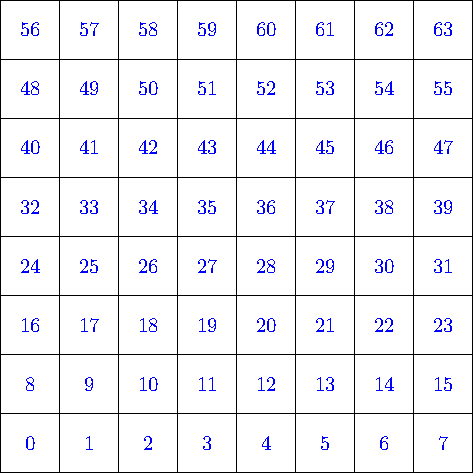
\includegraphics[width=40mm,angle=45]{images/grid8cm.pdf}
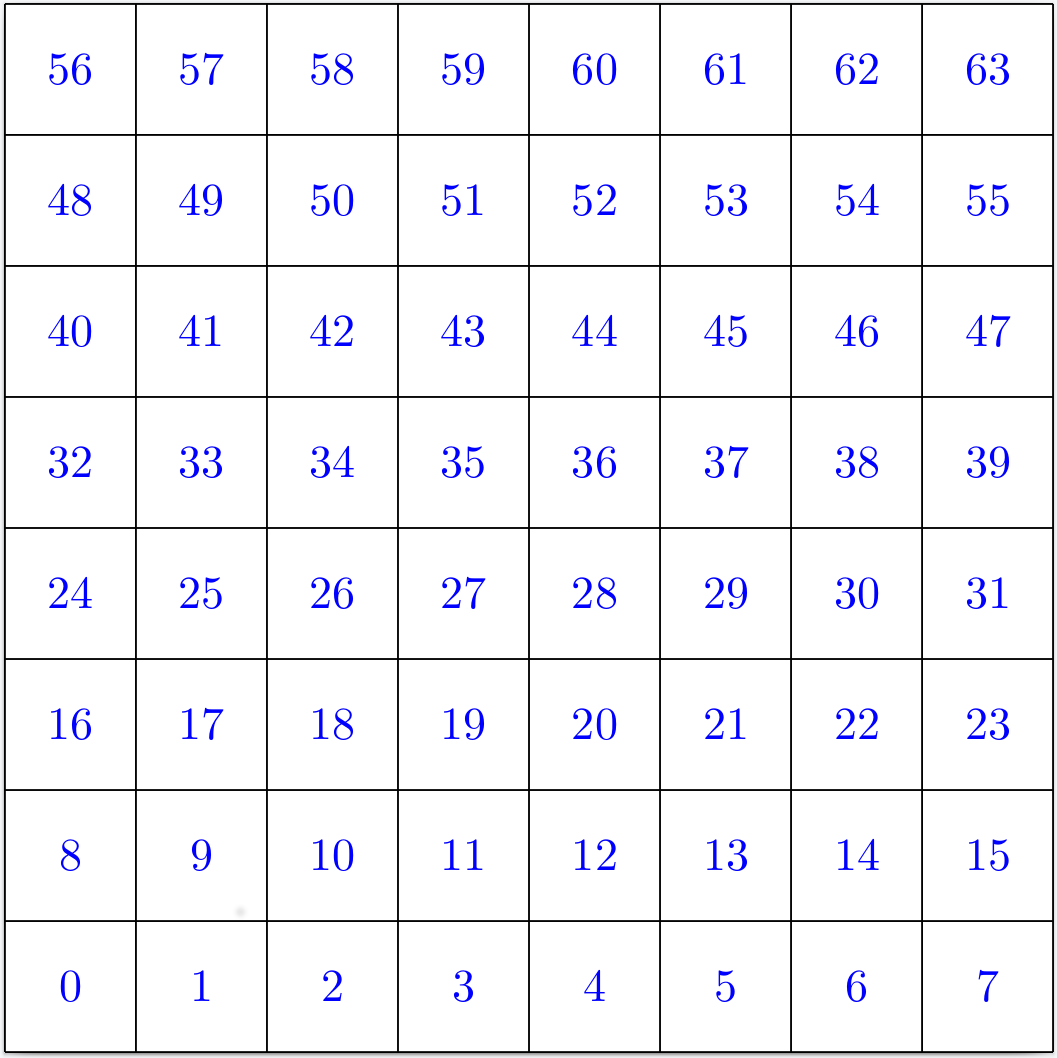
\includegraphics[angle=45,width=40mm]{images/grid8cm.png}
\end{verbatim}

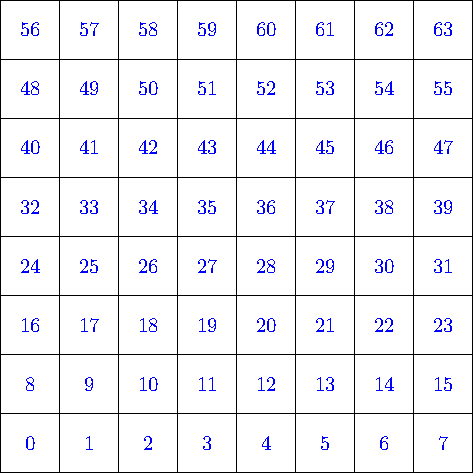
\includegraphics[width=40mm,angle=45]{images/grid8cm.pdf}
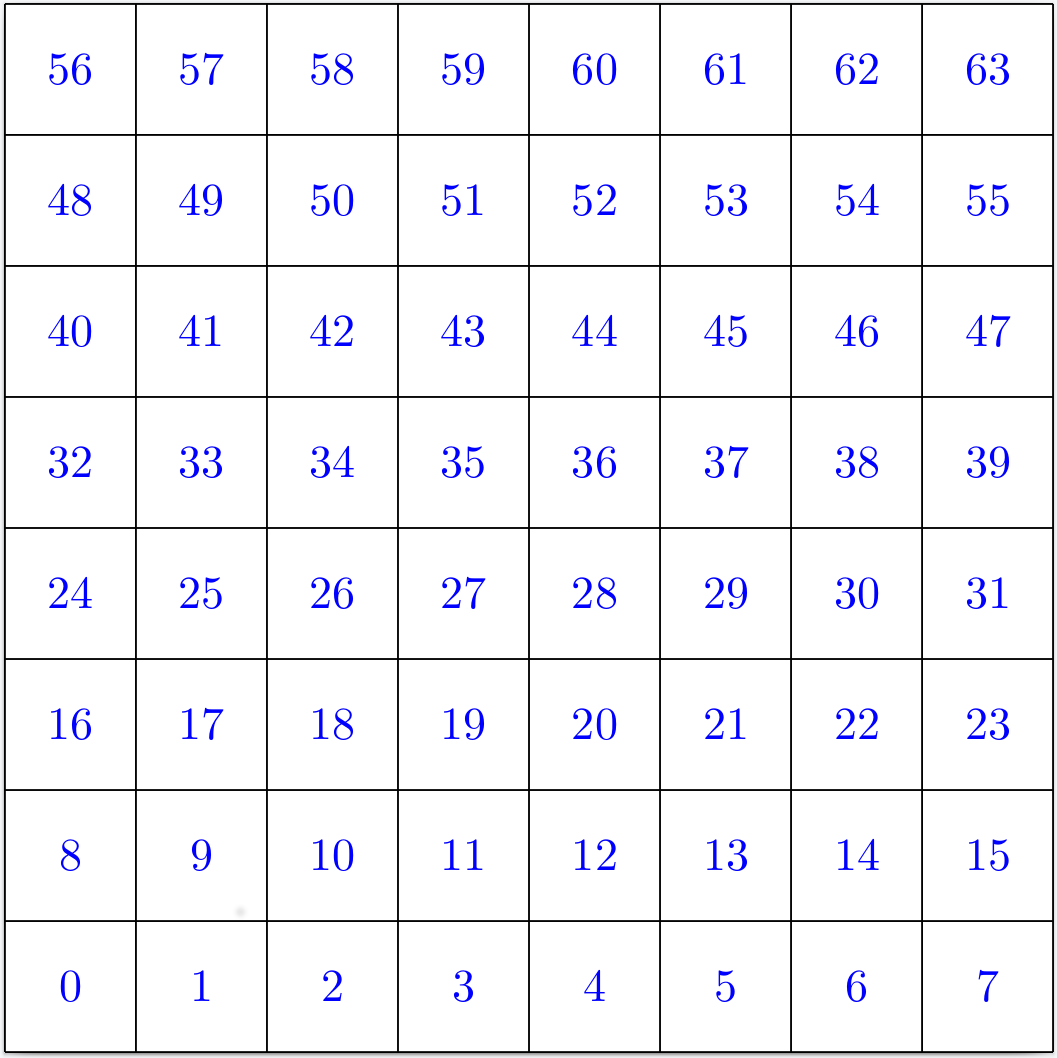
\includegraphics[angle=45,width=40mm]{images/grid8cm.png}

Also note that depending  on the resolution and zoom at  which you are viewing
this document, the lines  in the left image (which is the  PDF version) may or
may not show up on your screen. The PNG  version on the right does not seem to
suffer from this issue (at least for me).

For more options on rotations, consult the graphix manual.


% -------------------------------------------------------------------------- % 
\section{Getting an Image's True Size}
\label{sec:true-size}
% -------------------------------------------------------------------------- % 

\begin{minipage}[t][][b]{0.65\textwidth}
    Knowing the true size of a picture can relevant be when trying to clip it,
    so a quick overview  on the issue is presented here. A  way around this by
    using relative coordinates is presented in Section \ref{sec:rviewport}.

    There  are several  ways which  can be  used to  determine the  size of  a
    picture as  it would be  on the  page. One option is  to open the  file in
    an  image  editor  such  as  Gimp, Photoshop  or  similar,  and  view  its
    properties. For example,  the PNG  version of the  grid image  from above,
    \code{grid8cm.png},  opened in  Gimp,  gives the  following properties  as
    displayed in the picture to the right.

    Alternatively, one can  use the \code{extractbb} command  from the command
    line:
    \begin{verbatim}
$ extractbb imgages/grid8cm.png -O
    \end{verbatim}

    Which will yield:
    \begin{verbatim}
%%Title: images/grid8cm.png
%%Creator: extractbb 20160307
%%BoundingBox: 0 0 1061 1058
%%HiResBoundingBox: 0.000000 0.000000 1061.000000 1058.000000
%%CreationDate: Tue Mar 21 22:14:38 2017
    \end{verbatim}
\end{minipage}
\hfill
\begin{minipage}[t][][b]{0.3\textwidth}
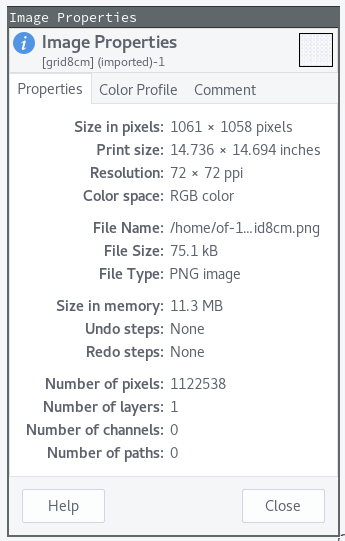
\includegraphics[width=\textwidth]{images/img-props.png}
\end{minipage}

\code{extractbb} also has other options; type \code{extractbb -h} for a list.
The \code{HiResBoundingBox} line in \code{extractbb}'s output will gives the
bounding box in points\footnotemark. For the PNG version of our grid, this
amounts to:

\footnotetext{$1\,\mathrm{pt} = 1/72\,\mathrm{in} 0.352\overline{7}\,\mathrm{mm}$}

\begin{center}
\begin{tabular}{rrrr}
    \toprule
    $0\,\mathrm{pt}$ & $0\,\mathrm{pt}$ & $1061\,\mathrm{pt}$ & $1058\,\mathrm{pt}$ \\
    \SI{0}{\milli\meter} & \SI{0}{\milli\meter} & \SI{374.3}{\milli\meter} & \SI{373.2}{\milli\meter} \\
    \bottomrule
\end{tabular}
\end{center}


% -------------------------------------------------------------------------- % 
\newpage
\section{The \code{clip} Option}
% -------------------------------------------------------------------------- % 

If  parts  of  a  picture  are  to  be  hidden  (either  through  use  of  the
\code{viewport}  or  the  \code{trim}  option\footnotemark),  the  \code{clip}
option needs to be enabled:

\footnotetext{%
    There  exists  also the  \code{bb}  option,  but  at  least in  my  \TeX{}
    installation, I tended to get an error  message in my compile log about it
    not making sense  and it was replaced on-the-fly  with the \code{viewport}
    option. Probably I'm simply not smart enough to use it right.}

\begin{verbatim}
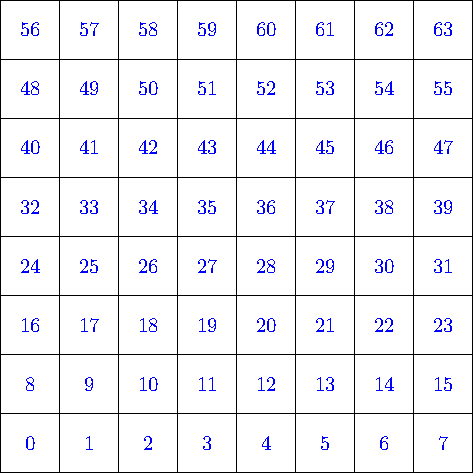
\includegraphics[clip,viewport=0 0 109 109]{images/grid8cm.pdf}
\end{verbatim}

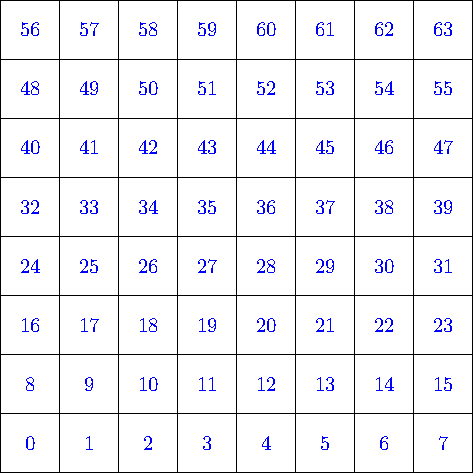
\includegraphics[clip,viewport=0 0 109 109]{images/grid8cm.pdf}

\vspace{2cm}

\textcolor{red}{Without the \code{clip} option set to \code{true}, this is what happens:}

\begin{verbatim}
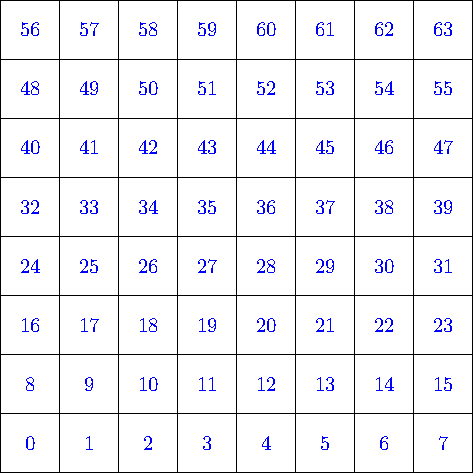
\includegraphics[bb=3cm 3cm 5cm 5cm]{images/grid8cm.pdf}
\end{verbatim}

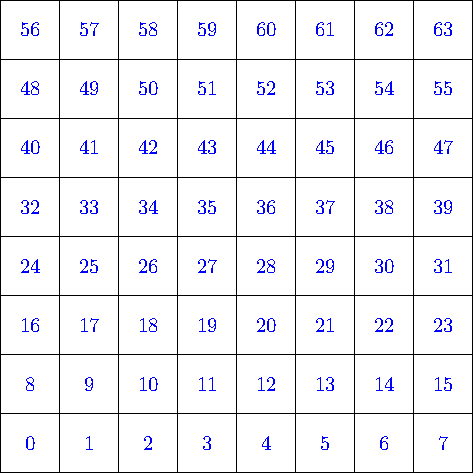
\includegraphics[bb=3cm 3cm 5cm 5cm]{images/grid8cm.pdf}

\textcolor{red}{Note where the next line of text continues.}

\vspace{3cm}

With the \code{clip} option, we get the desired result:

\begin{verbatim}
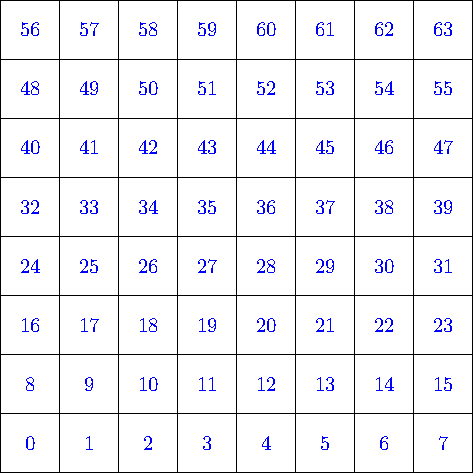
\includegraphics[clip,bb=3cm 3cm 5cm 5cm]{images/grid8cm.pdf}
\end{verbatim}

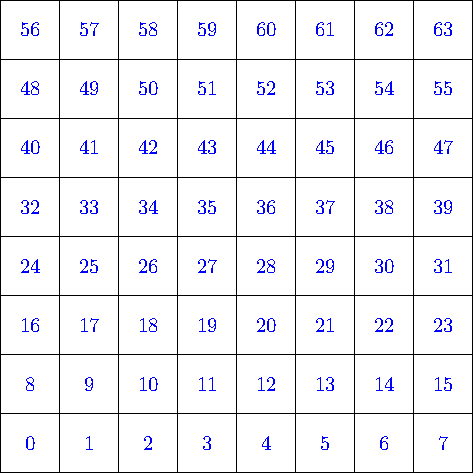
\includegraphics[clip,bb=3cm 3cm 5cm 5cm]{images/grid8cm.pdf}


% -------------------------------------------------------------------------- % 
\section{The \code{viewport} Option}
% -------------------------------------------------------------------------- % 

As seen above,  the \code{viewport} option can  be used to select  a region of
the included document's bounding box which is to be shown:

\begin{verbatim}
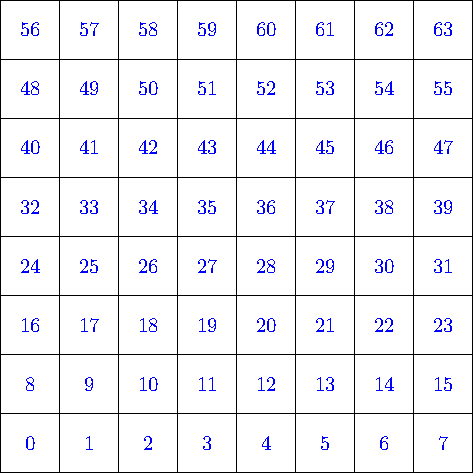
\includegraphics[clip=true,viewport=2cm 2cm 6cm 6cm]{images/grid8cm.pdf}
\end{verbatim}

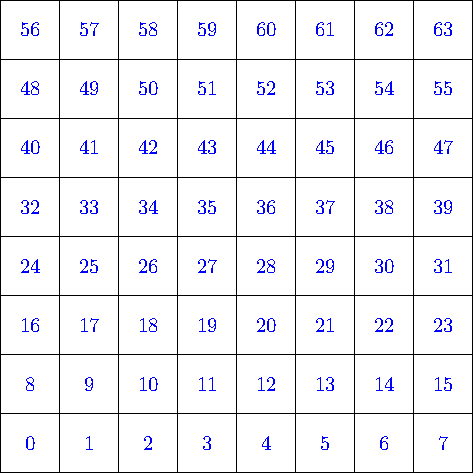
\includegraphics[clip=true,viewport=1cm 1cm 7cm 7cm]{images/grid8cm.pdf}

\vspace{1em}

The first, last, top and bottom rows and columns have been cut off.  The lines
at the  top and bottom  are not or only  partially displayed because  they are
just slightly outside  the \SI{7}{\centi\meter} bounding box  as we've defined
it.

Because the  frame of reference  is the  included document's bounding  box, an
optional \code{width} or \code{height} argument can be placed either before or
after the \code{viewport} option. The result will be the same.

\begin{verbatim}
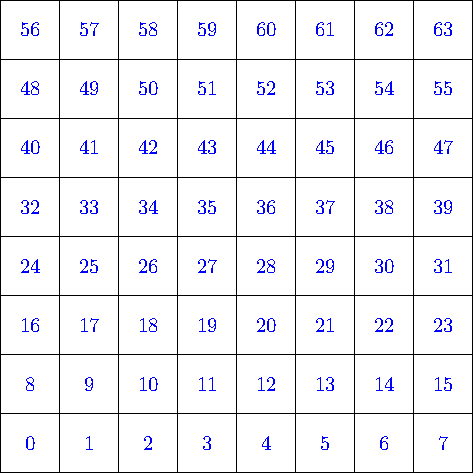
\includegraphics[width=30mm,clip=true,viewport=1cm 1cm 7cm 7cm]{images/grid8cm.pdf}
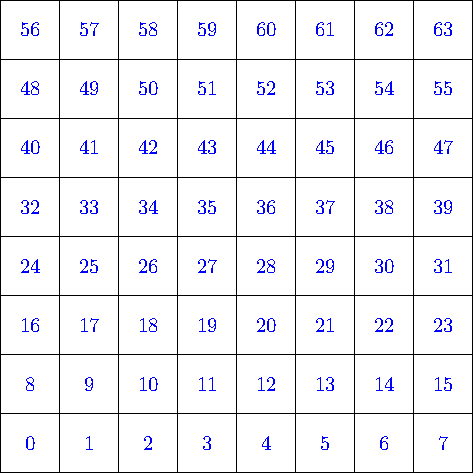
\includegraphics[clip=true,viewport=1cm 1cm 7cm 7cm,width=30mm]{images/grid8cm.pdf}
\end{verbatim}

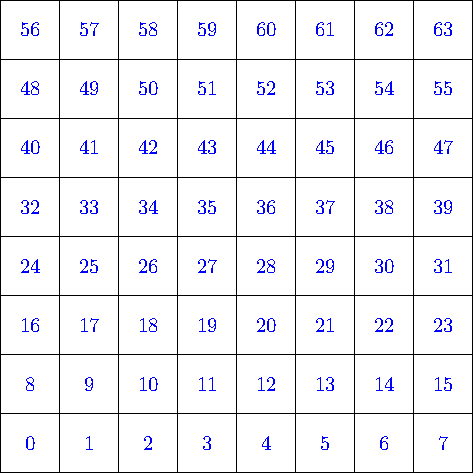
\includegraphics[width=30mm,clip=true,viewport=1cm 1cm 7cm 7cm]{images/grid8cm.pdf}
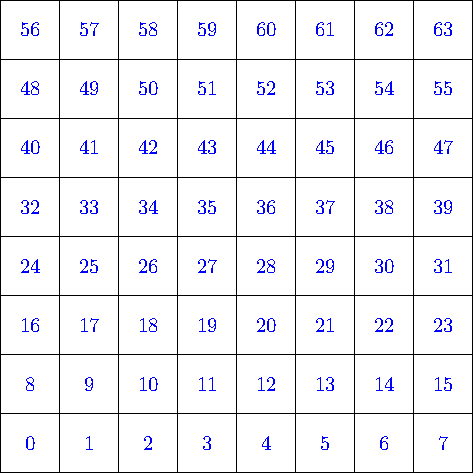
\includegraphics[clip=true,viewport=1cm 1cm 7cm 7cm,width=30mm]{images/grid8cm.pdf}

Another  effect of  the  \code{viewport}  argument being  in  relation to  the
included document's bounding box is that in  case of the PNG version, we get a
rather different  result, because it is  significantly larger, as we  found in
Section \ref{sec:true-size}.

\begin{verbatim}
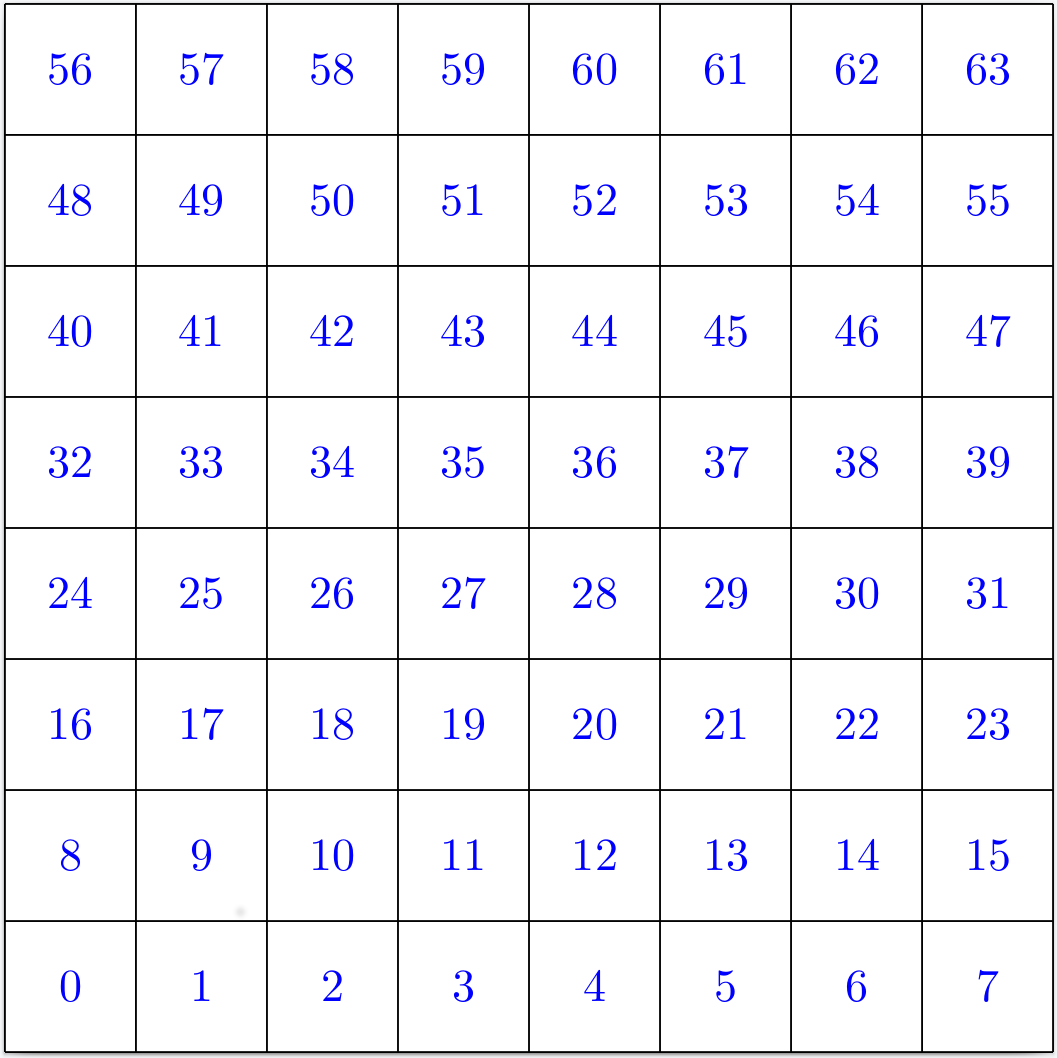
\includegraphics[clip=true,viewport=1cm 1cm 7cm 7cm,width=30mm]{images/grid8cm.png}
\end{verbatim}

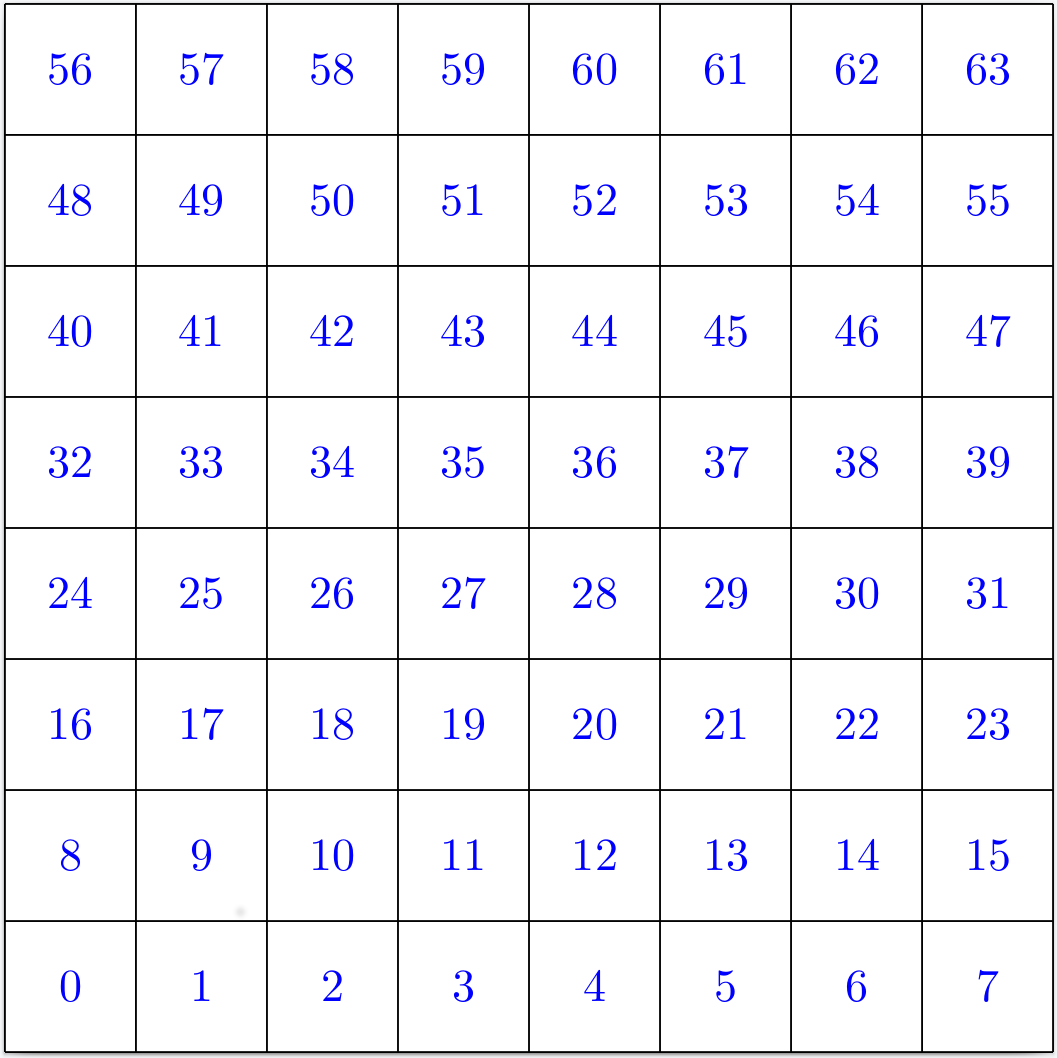
\includegraphics[clip=true,viewport=1cm 1cm 7cm 7cm,width=30mm]{images/grid8cm.png}


% -------------------------------------------------------------------------- % 
\newpage
\section{The \code{trim} Option}
% -------------------------------------------------------------------------- % 

The  \code{trim}  option, instead  of  selecting  a  region from  an  included
document which is to  be shown, selects regions of said  document which are to
be cut off. Also,  again, the parameters passed to the  \code{trim} option are
in relation to the included document's  size, and we get different results for
the PDF  and PNG  versions due  to their  different sizes. However,  both have
\SI{1}{\centi\meter} clipped on all four sides.

\begin{verbatim}
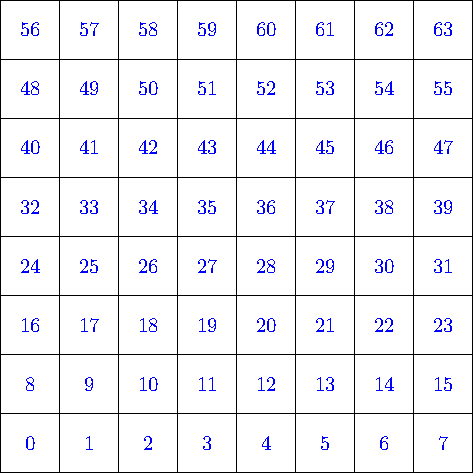
\includegraphics[width=0.5\textwidth,clip=true,trim=1cm 1cm 1cm 1cm]{images/grid8cm.pdf}
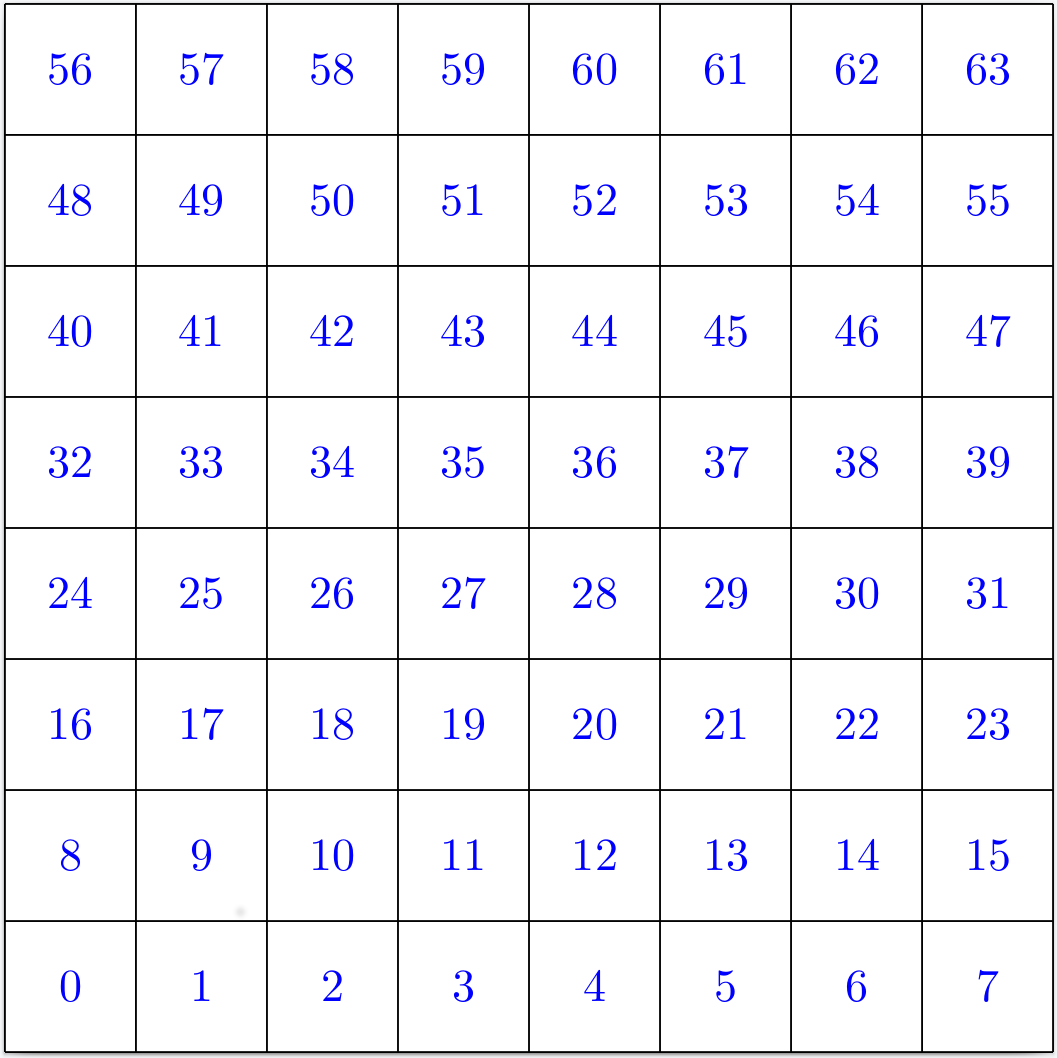
\includegraphics[width=0.5\textwidth,clip=true,trim=1cm 1cm 1cm 1cm]{images/grid8cm.png}
\end{verbatim}

\noindent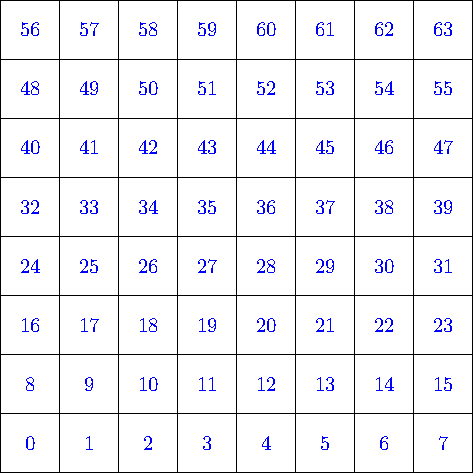
\includegraphics[width=0.5\textwidth,clip=true,trim=1cm 1cm 1cm 1cm]{images/grid8cm.pdf}
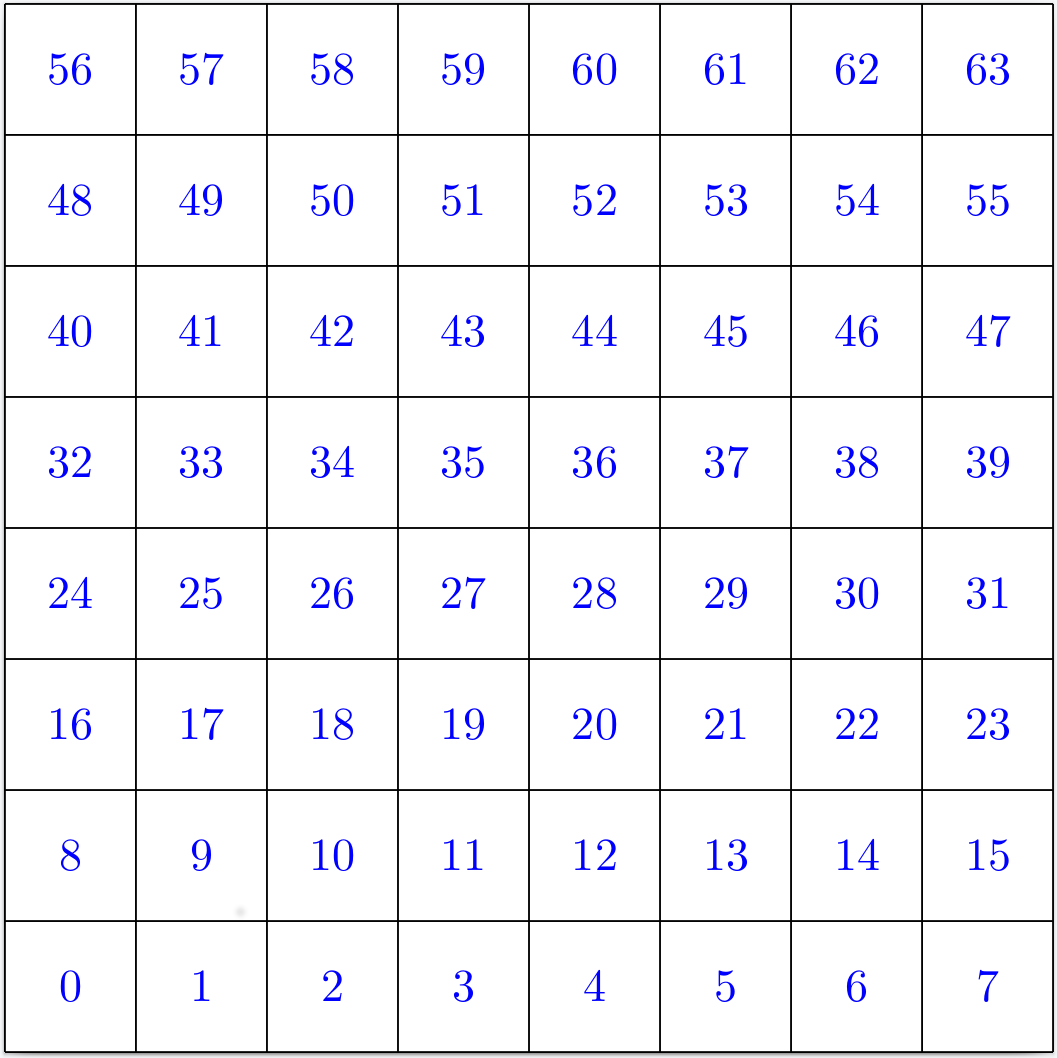
\includegraphics[width=0.5\textwidth,clip=true,trim=1cm 1cm 1cm 1cm]{images/grid8cm.png}


% -------------------------------------------------------------------------- % 
\newpage
\section{The \code{rviewport} Package}
\label{sec:rviewport}
% -------------------------------------------------------------------------- % 

The \code{rviewport}\footnotemark  package allows to use  relative coordinates
instead of absolute coordinates to specify the areas which are to be clipped.

\footnotetext{
    Package documentation available at:
    \href{https://www.ctan.org/pkg/rviewport}{\nolinkurl{https://www.ctan.org/pkg/rviewport}}}

\begin{verbatim}
% Preamble:
\usepackage{rviewport}
% Document
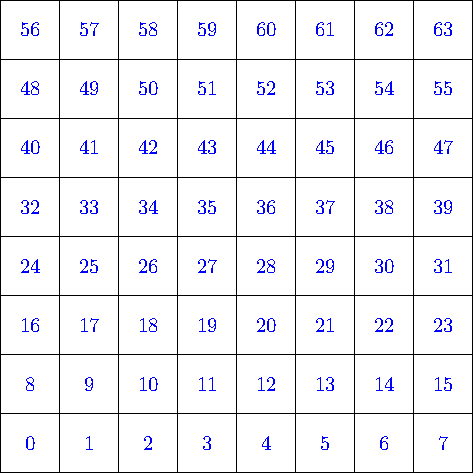
\includegraphics[clip,rviewport=0.125 0.125 0.875 0.875]{images/grid8cm.pdf}
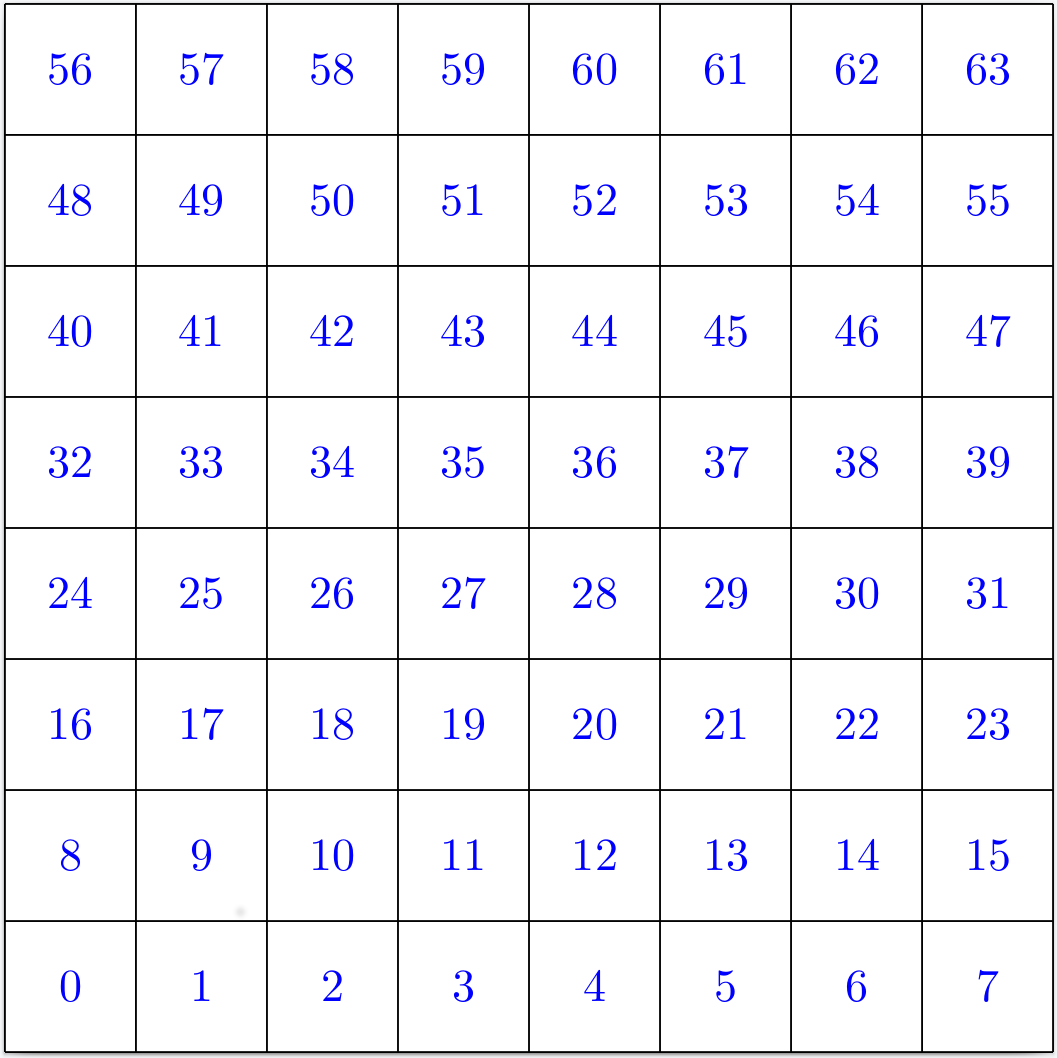
\includegraphics[width=6cm,clip,rviewport=0.125 0.125 0.875 0.875]{images/grid8cm.png}
\end{verbatim}

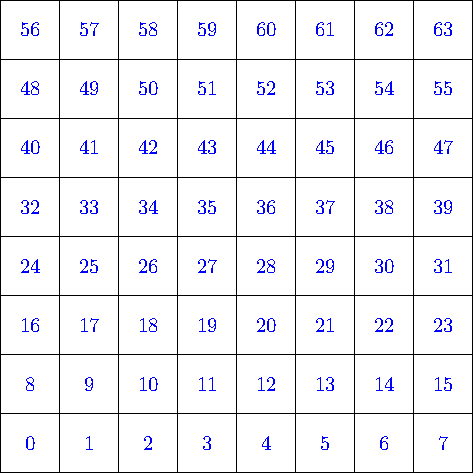
\includegraphics[clip,rviewport=0.125 0.125 0.875 0.875]{images/grid8cm.pdf}
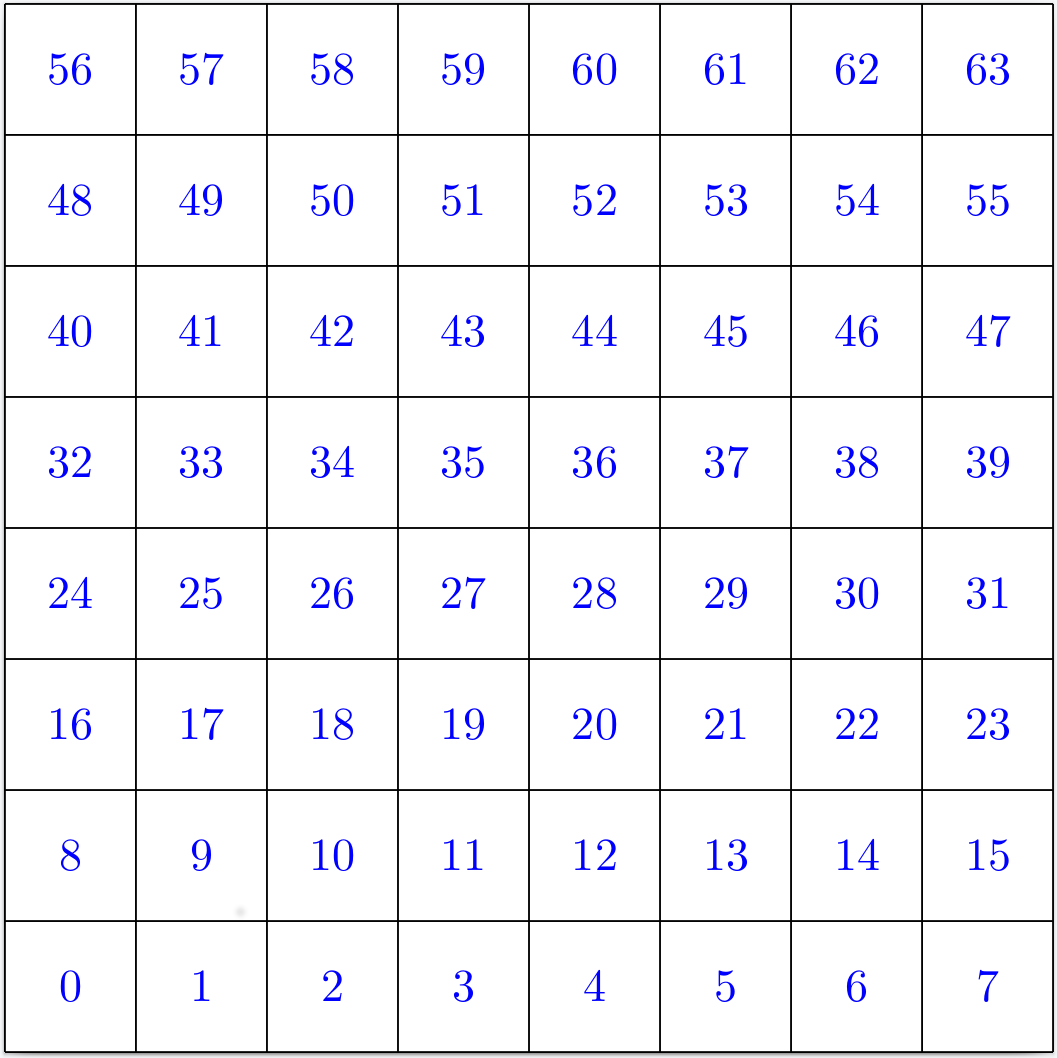
\includegraphics[width=6cm,clip,rviewport=0.125 0.125 0.875 0.875]{images/grid8cm.png}

\end{document}
